\chapter{Equivalência e Ordem}\label{cap:EquivalenciaOrdem}

\epigraph{``Matemática não é difícil, matemática tem muita lógica e o que é lógico não pode ser difícil''.}{João Lucas Marques Barbosa}

\epigraph{``O grande inimigo do conhecimento não é a ignorância, é a ilusão de ter conhecimento''.}{Stephen Hawking}

%\epigraph{``O problema do mundo hoje é que as pessoas inteligentes estão cheias de dúvidas, e as pessoas idiotas estão cheias de certezas...''}{Bertrand Russell}`

\section{Introdução}\label{sec:IntroEquivalenciaOrdem}

No Capítulo \ref{cap:Relacoes} anterior este manuscrito apresentou ao leitor a ideia de relações entre conjuntos, em especial foram tratadas as relações binários sobre um conjunto dado. Agora nesta seção será apresentada de forma mais profunda as relações de equivalência. Como dito em \cite{abe1991-TC, carmo2013}, as relações de equivalência ao lado das relações de ordem (estudadas na Seção \ref{sec:Ordem}) são de importante central para toda a matemática, além disso, as relações de equivalência também desempenho importantes papéis nas área de mineração de dados \cite{lin1999data, lingras1998data}, aprendizado de máquina \cite{bar2003learning} e processamento de sinais \cite{li2007equivalent} e imagens \cite{acharya2003classification, myasnikov2018description}. E por sua vez, as relações de ordem também aparecem em diversas áreas de caráter prática tais como processamento de imagens \cite{farias2016image, cressie1998image}, criptografia \cite{giri2008crypto}, otimização \cite{karaman2018partial} e etc.

\section{Relações de Equivalência e Espaço Quociente}\label{sec:Equivalencia}

Mas o que seria uma relação de equivalência? Bem, uma resposta satisfatória para essa pergunta é que uma relação de equivalência pode ser entendida como sendo uma forma de parear os elementos de um conjunto que apresentam similaridade entre si com respeito a uma ou mais propriedades específicas, isto é, uma relação de equivalência junta os elementos em pares pela similaridade deles. A seguir será apresentado de forma precisa o conceito de relação de equivalência.

\begin{definition}[Relação de Equivalência]\label{def:RelacaoEquivalencia}
	Seja $A$ um conjunto uma relação binária $\equiv$ sobre $A$ é dita ser uma relação de equivalência sempre que $\equiv$ for reflexiva, simétrica e transitiva.
\end{definition}

\begin{remark}
	Como dito em \cite{carmo2013} além da notação $\equiv$ outros símbolos também são comumente encontrados na literatura para representar relações de equivalência, entre, tais símbolos destacam-se $\approx$ e $\sim$. Neste manuscrito tais símbolos apareceram mais adiante representando outros conceitos, assim neste manuscrito será usado sempre usado o símbolo $\equiv$, a menos que seu uso gere confusão e nesse caso será usado notações como $R_i$ para denotar relação de equivalência, em que $i$ poderá ser um número natural ou o rótulo de um conjunto.
\end{remark}

\begin{example}\label{exe:Equivalencia1}
	Dado um conjunto $C$ qualquer, a relação de igualdade $(=)$ definida em $C$ é obviamente uma relação de equivalência.
\end{example}

\begin{example}\label{exe:Equivalencia2}
	Dado o conjunto $A =\{a, b, c, d\}$ a relação definida por $a \equiv a$, $a \equiv b$, $b \equiv a$, $b \equiv b$, $c \equiv c$ e $d \equiv d$, é claramente uma relação de equivalência.
\end{example}

Os Exemplos \ref{exe:Equivalencia1} e \ref{exe:Equivalencia2} permite o leitor perceber uma importante verdade matemática, tal verdade como expressa em \cite{carmo2013} pode ser escrita como: ``objetos iguais são equivalentes, mas objetos equivalentes nem sempre são iguais''.

\begin{example}
	Dado um plano $P$ a relação de paralelismo definido sobre o conjunto de retas de $P$ é uma relação de equivalência, outro exemplo clássico da geometria é a semelhança entre triângulos neste mesmo plano $P$.
\end{example}

\begin{example}
	A relação $R = \{(x, y) \in \mathbb{N}^2 \mid x, y \text{ possuem o mesmo resto da divisão por } 5\}$ é um relação de equivalência.
\end{example}

\begin{example}
	A relação $I =  \{(x, y) \in PERS^2 \mid x, y \text{ possuem a mesma idade}\}$ é um relação de equivalência sobre o conjunto de todas as pessoas $(PERS)$.
\end{example}

\begin{example}
	Dado o conjunto de todos os times de futebol do Brasil a relação $T$ definida como $x \mathrel{T} y \Longleftrightarrow x, y \text{ nunca foram rebaixados para a segunda divisão}$, é uma relação de equivalência.
\end{example}

%A partir da noção de relação de equivalência é possível como destacado em \cite{abe1991-TC} definir a noção de classes de equivalência. 

\begin{definition}[Classes de Equivalência]
	Seja $\equiv$ uma relação de equivalência sobre um conjunto $A$, para todo $x \in A$ é definida a classe de equivalência de $x$, denotado por $[x]$, como sendo o conjunto de todos os elementos equivalentes a $x$, simbolicamente tem-se que:
	$$[x] = \{y \in A \mid y \equiv x\}$$
\end{definition}

Obviamente toda classe de equivalência $[x]$ é um subconjunto do conjunto base\footnote{Conjunto base aqui diz respeito ao conjunto sobre o qual a relação de equivalência está definida.}. Além disso,  obviamente tem-se que $[x] = \emptyset$ se, e somente se, o conjunto base for vazio. 

\begin{example}\label{exe:ClasseEquivalencia1}
	Seja $A = \{0, 1, 2, 3\}$ e $0 \equiv 0$, $1 \equiv 1$, $2 \equiv 2$, $3 \equiv 3$, $0 \equiv 2$, $1 \equiv 3$, $2 \equiv 0$, $3 \equiv 1$ tem-se que: $[0] = \{0, 2\}$, $[1] = \{1, 3\}$, $[2] = \{0, 2\}$ e $[3] = \{1, 3\}$.
\end{example}

\begin{example}
	A relação $a \equiv a$, $b \equiv b$, $c \equiv c$, $a \equiv b$, $b \equiv a$ definida sobre o conjunto $\{a, b, c\}$ é uma relação de equivalência e existem as seguintes classes de equivalência $[a] = [b] = \{a, b\}$ e $[c] =\{c\}$.
\end{example}

\begin{theorem}\label{teo:EquivalenciaPropriedade1}
	Seja $\equiv$ uma relação de equivalência sobre um conjunto $A$ não vazio e sejam $a, b \in A$ tem-se que $a \equiv b$ se, e somente se, $[a] = [b]$.
\end{theorem}

\begin{proof}
	$(\Rightarrow)$ Suponha que $a \equiv b$, assim dado  qualquer $x \in [a]$ tem-se que $x \equiv a$, agora pela transitiva de $\equiv$ é claro que $x \equiv b$ e, portanto, $x \in [b]$, logo $[a] \subseteq [b]$ e com raciocínio similar pode-se concluir que $[b] \subseteq [a]$ e assim pela Definição \ref{def:IgualdadeConjuntos} tem-se que $[a] = [b]$. $(\Leftarrow)$ Suponha que $[a] = [b]$, por $\equiv$ ser reflexiva é claro que $a \equiv a$ e assim $a \in [a]$, mas como $[a] = [b]$ tem-se que $a \in [b]$, e portanto, por definição $a \equiv b$.
\end{proof}

\begin{theorem}\label{teo:EquivalenciaPropriedade2}
	Seja $\equiv$ uma relação de equivalência sobre um conjunto $A$ não vazio e sejam $a, b \in A$ tem-se que $a \not\equiv b$ se, e somente se, $[a] \cap [b] = \emptyset$.
\end{theorem}

\begin{proof}
	$(\Rightarrow)$ Suponha por absurdo que $a \not\equiv b$ e $[a] \cap [b] \neq \emptyset$, logo existe um $x \in A$ tal que $x \in [a] \cap [b]$, mas assim pela Definição \ref{def:IntersecaoConjuntos} tem-se que $x \in [a]$ e $x \in [b]$, logo $x \equiv a$ e $y \equiv b$, mas uma vez que $\equiv$ é simétrica tem-se que $a \equiv x$, e como $\equiv$ é transitiva tem-se que $a \equiv b$, o que contradiz a hipótese, caraterizando um absurdo, consequentemente, se $a \not\equiv b$ tem-se então que $[a] \cap [b] = \emptyset$. $(\Leftarrow)$ Suponha que $[a] \cap [b] = \emptyset$, como $a \in [a]$ e pela hipótese $a \notin [a] \cap [b]$ tem-se que $a \notin [b]$ e, portanto, $a \not\equiv b$.
\end{proof}

\begin{definition}[Espaço Quociente]
	Seja $A$ um conjunto e $\equiv$ uma relação de equivalência sobre $A$, o espaço quociente de $A$ com respeito (ou módulo) $\equiv$, denotado por $A_{/_\equiv}$, é o conjunto de todas as classes de equivalência do conjunto $A$, na linguagem na teoria dos conjuntos tem-se que:
	$$A_{/_\equiv} = \{[x] \mid x \in A\}$$
\end{definition}

\begin{example}
	Seja $A = \{1, 2, 3\}$ e $R = \{(a, a), (b, b), (c, c), (a, b), (b, a)\}$ claramente $R$ é uma relação de equivalência e além disso $[a] = [b] = \{a, b\}$ e $[c] = \{c\}$ assim $A_{/_R} = \{[a], [c]\}$.
\end{example}

\begin{example}
	Dado que a relação $P = \{(x,y) \in \mathbb{Z}_+ \mid x, y\text{ tem o mesmo resto da divisão por } 2\}$ é uma relação de equivalência sobre $\mathbb{Z}_+$ (a prova fica como exercício ao leitor) tem-se claramente que, 
	$$[0] = \{0, 2, 4, 6, 8, \cdots\}$$
	e
	$$[1] = \{1, 3, 5, 7, 9, \cdots\}$$
	ou seja, $[0]$ é o conjunto dos pares positivos e $[1]$ é o conjunto dos impares positivos, assim claramente tem-se que $\mathbb{Z}_{+/_P} = \{[0], [1]\}$.
\end{example}

Uma fato importante sobre o espaço quociente de uma relação de equivalência $\equiv$ é que sempre que o conjunto base $A \neq \emptyset$ tem-se que $A_{/_\equiv} \neq \emptyset$, e mais do que isso, como mostrado a seguir o espaço quociente é sempre uma partição sobre o conjunto base $A$.

\begin{theorem}
	Seja $\equiv$ uma relação de equivalência sobre um conjunto não vazio $A$, então $A_{/_\equiv}$ é uma partição de $A$.
\end{theorem}

\begin{proof}
	Primeiramente note que como $\equiv$ é uma relação reflexiva tem-se para todo $x \in A$ que $x \in [x]$ e assim claramente $[x] \in A_{/_\equiv}$ e $[x] \neq \emptyset$, satisfazendo assim a condição (1) da Definição \ref{def:ParticaoConjuntos}. Por outro lado, os Teoremas \ref{teo:EquivalenciaPropriedade1} e \ref{teo:EquivalenciaPropriedade2} mostram que dado $[x], [y] \in A_{/_\equiv}$ sempre que $[x] \neq [y]$ tem-se que  $[x] \cap [y] = \emptyset$ e, portanto, a condição (2) da Definição \ref{def:ParticaoConjuntos} é satisfeita, desde que as condições (1) e (2) são satisfeita pelo elementos de $A_{/_\equiv}$ tem-se que $A_{/_\equiv}$ é uma partição de $A$.
\end{proof}

Um interessante uso das relações de equivalência é como dito em \cite{carmo2013} a construção do conjunto dos números racionais $(\mathbb{Q})$ a partir dos números inteiros $(\mathbb{Z})$.

%Um interessante uso das relações de equivalência é como dito em \cite{carmo2013} a construção do conjunto dos números racionais $(\mathbb{Q})$ a partir dos números inteiros $(\mathbb{Z})$, para o leitor interessando tal construção está detalhada no apêndice \ref{ape:Racionais}.

\section{Relações de Ordem}\label{sec:Ordem}

Em algumas situação é interessante que seja possível definir uma hierarquia entre os elementos de um determinado conjunto, de fato, como dito em \cite{abe1991-TC} diversos campos das ciências empíricas, tais como a área da biologia comparada, são dependentes de construções hierárquicas. Dentro da própria ciência da computação diversas áreas (estrutura de dados, classificação de dado e etc.) também utilizam de ordens de hierarquia. Assim é conveniente apresentar o estudo das relações de ordem e das estruturas existentes envolta de tais relações, para isso apresenta-se primeiro as ideias de pré-ordem e ordem estrita.

\begin{definition}[Ordem Estrita]\label{def:OrdemParcialEstrita}
	Seja $A$ um conjunto uma relação $\sqsubset$ sobre $A$, é dita ser uma relação de ordem parcial estrita, ou simplesmente ordem estrita, sempre que $\sqsubset$ for irreflexiva e transitiva.
\end{definition}

\begin{example}
	A relação $\{(x, y) \in \mathbb{N}^2 \mid y = x + 1\}$ é uma ordem estrita.
\end{example}

\begin{example}
	Dado um conjunto $A$ qualquer a relação de ser subconjunto próprio $(\subset)$ é um ordem estrita sobre o conjunto $\wp(A)$.
\end{example}

\begin{example}
	Dado o conjunto $\{1, 2, 3\}$ a relação $\{(1, 2), (2, 3), (2, 2), (1, 3)\}$ não é uma ordem estrita pois $(2, 2)$ é um par pertencente a relação.
\end{example}

\begin{definition}[Pré-ordem]
	Seja $A$ um conjunto uma relação $\sqsubseteq$ sobre $A$, é dita ser uma relação de pré-ordem sempre que $\sqsubseteq$ for reflexiva e transitiva.
\end{definition}

\begin{example}
	Dado o conjunto $\{a, b, c\}$ a relação $\{(a, a), (b, b), (c, c), (b, c), (c, a), (b, a)\}$ é uma relação de pré-ordem.
\end{example}

\begin{example}
	A relação $\{(x, y) \in \mathbb{N}^2 \mid (\exists x \in \mathbb{N})[y = xk]\}$ é uma pré-ordem.
\end{example}

\begin{example}
	A relação $\{(x, y) \in \mathbb{N}^2 \mid x + y \neq x \text{ e } x + y \neq y\}$ não é uma pré-ordem pois não é reflexiva, basta notar que $(0,0)$ não pertence a tal relação.
\end{example}

Aumentando as restrições sobre uma pré-ordem, isto é, adicionando mais propriedades a serem exigidas, é construída a noção de ordem parcial, tal conceito é formalizado a seguir. 

\begin{definition}[Ordem Parcial]\label{def:OrdemParcial}
	Seja $A$ um conjunto uma relação $\sqsubseteq$ sobre $A$, é dita ser uma relação de ordem parcial sempre que $\sqsubseteq$ for reflexiva, antissimétrica e transitiva.
\end{definition}

Como dito em \cite{abe1991-TC} se $\sqsubseteq$ é uma ordem parcial sobre um conjunto $A$, então tem-se que $\sqsubseteq$ organizar (ou ordena) o conjunto $A$ em uma determinada hierarquia (ou ordem), obviamente um mesmo conjunto pode apresentar diferentes ordenações, ou seja, podem existir diversas ordens parciais sobre $A$.

\begin{remark}\label{rema:SematicaOrdemParcial}
	De forma geral quando $x \sqsubseteq y$ pode ser interpretado como $x$ é anterior ou igual a $y$, entretanto, para o caso especifico das relações de ordem parcial $\leq$ e $\subseteq$ suas semânticas sãos as aquelas que o leitor já conhece, isto é, $x \leq y$ significa $x$ é menor ou igual a $y$ e $X \subseteq Y$ significa que $X$ é subconjunto de $Y$.
\end{remark}

Além das duas famosas ordens parciais mencionadas na Observação \ref{rema:SematicaOrdemParcial} a seguir serão apresentados mais algumas ordens parciais.

\begin{example}\label{exe:OrdemParcialSimples}
	As seguintes relações são exemplos de ordens parciais:
	\begin{itemize}
		\item[(a)] $\{(x, y) \in \mathbb{N}^2 \mid (\exists k \in \mathbb{N})[y = x + k]\}$.
		\item[(b)] $\{(x, y) \in \mathbb{N}^2 \mid (\exists k \in \mathbb{N})[y = xk]\}$.
		\item[(c)] Dado um conjunto $A$ de todas as pessoas da terra a relação $x \mathrel{R} y$ se, e somente se, $x$ tem a mesma altura ou é mais alto que $y$, é uma ordem parcial sobre $A$.
	\end{itemize}
\end{example}

\begin{remark}
	O leitor atendo pode notar que a ordem no item $(b)$ do Exemplo \ref{exe:OrdemParcialSimples} foi anteriormente usado como exemplo de uma pré-ordem, isso ocorre por que toda ordem parcial é uma pré-ordem.
\end{remark}

\begin{example}
	Seja $A = \{a, b, c, d\}$ a relação $\{(a, a), (b, b), (c, c), (d, d), (a, b), (b, c), (a, c), (a, d)\}$ é uma ordem parcial sobre $A$.
\end{example}

\begin{example}
	Dado o $\{0,1\}$ a relação $\{(0,0), (0, 1), (1, 1)\}$ é uma ordem parcial.
\end{example}

\begin{example}
	Dado um conjunto $\{0, 1, 2, 3\}$ a relação $\{(0, 0), (0, 1), (2, 2), (1, 2), (0, 2), (3, 3)\}$ não é um ordem parcial pois o par $(1, 1)$ não pertence a relação e por definição uma ordem parcial deve ser reflexiva.
\end{example}

A partir da ideia de ordem parcial é possível definir o conceito de comparabilidade como se segue.

\begin{definition}[Comparabilidade]\label{def:Comparabilidade}
	Seja $A$ um conjunto não vazio, $\sqsubseteq$ uma ordem parcial sobre $A$ e seja $x, y \in A$, é dito que $x$ e $y$ são comparáveis sempre que $x \sqsubseteq y$ ou $y \sqsubseteq x$.
\end{definition}

Como dito em \cite{abe1991-TC, carmo2013} tem-se que a noção de comparabilidade está ligada a ordem em questão, assim pode haver um conjunto $A$ e uma ordem parcial $\sqsubseteq_1$ tal que dois elementos $x$ e $y$ são comparáveis, entretanto, pode haver outra ordem parcial $\sqsubseteq_2$ sobre o mesmo conjunto tal que os elementos $x$ e $y$ não pode ser comparáveis\footnote{Em algumas obras é usado a escrita $x \not\sqsubseteq y$ para esboça que $x$ e $y$ são incomparáveis por uma ordem parcial $\sqsubseteq$.}.

\begin{example}
	Considere o conjunto $A = \{1, 2, 3\}$ tem-se que $\subseteq$ será obviamente um ordem parcial sobre $\wp(A)$, agora note que $\{1, 2\} \subseteq A$, portanto, $\{1, 2\}$ e $A$ são comparáveis, por outro lado, $\{1, 2\} \not\subseteq \{1, 3\}$ e $\{1, 3\} \not\subseteq \{1, 2\}$, logo $\{1, 2\}$ e $\{1, 3\}$ são incomparáveis.
\end{example}

\begin{example}
	Dado o conjunto $\mathbb{R}$ e a ordem parcial $\leq$ sobre $R$ tem-se que todo par de números reais $(x, y)$ é sempre comparável.
\end{example}

Por fim é apresentado a ideia de ordem parcial, pela definição a seguir é fácil para o leitor perceber que toda ordem total é uma ordem parcial, porém, o oposto não é verdade.

\begin{definition}[Ordem total]
	Uma ordem parcial $\sqsubseteq$ sobre um conjunto $A$ é dita ser total quando para todo par de elementos $x, y \in A$ é comparável.
\end{definition}

\begin{example}
	São exemplos de ordem totais:
	\begin{itemize}
		\item[(a)] A ordem usual ``menor igual'' $(\leq)$ sobre o conjunto $\mathbb{R}$.
		\item[(b)] A relação $\{(a_0, a_0), (a_0, a_1), (a_0, a_2), (a_1, a_1), (a_1, a_2), (a_2, a_2)\}$ sobre o conjunto $\{a_0, a_1, a_2\}$.
	\end{itemize}
\end{example}

Nesta seção ao apresentar a ideia de relações de ordem isso era feito pelo estudo da relação em si ficando seu conjunto base em segundo plano e com pouco interesse, agora será considera simultaneamente os dois conceitos juntos, ou seja, será agora apresentado o conceito de conjunto parcialmente ordenado.

\section{\textit{Posets} e Diagramas de Hasse}\label{sec:Poset}

Como dito em \cite{neggers1998poset},  os conjuntos parcialmente ordenados ou \textit{posets} (em inglês) têm uma longa história que remonta ao início do século XIX, onde as propriedades da ordenação dos subconjuntos de um conjunto foram investigadas.  Embora o matemático Felix Hausdorff\footnote{Famoso por seus trabalhos em topologia.} (1868-1942) não tenha sido a pessoa que introduziu a ideia de conjunto parcialmente ordenado, foi ele que fez o primeiro estudo sério de uma teoria geral dos posets em seu trabalho \cite{hausdorff1914poset}. 

\begin{definition}[Poset]
	Um conjunto parcialmente ordenado ou \textit{poset} é uma estrutura $\langle A, \sqsubseteq \rangle$ onde $A$ é um conjunto não vazio e $\sqsubseteq$ é uma ordem parcial sobre $A$.
\end{definition}

\begin{example}
	São exemplos de conjuntos parcialmente ordenados:
	\begin{itemize}
		\item[(a)] $\langle \wp(A), \subseteq \rangle$.
		\item[(b)] $\langle C,  : \rangle$ onde $C = \{1, 2, 3, 4, 5, 6, 12\}$ e $x : y$ se, e somente se, $x$ é um divisor de $y$.
		\item[(c)] $\langle \mathbb{Z}, \geq \rangle$.
		\item[(d)] $\langle B, \subseteq \rangle$ onde $B = \{R_1, R_2, \cdots\}$ é o conjunto de todas as relações binárias sobre um conjunto $A$.
	\end{itemize}
\end{example}

Agora como dito em \cite{morgado1962poset}, muitas vezes é conveniente utilizar uma representação gráfica para os \textit{posets} que possa evidenciar as relações hierárquicas existentes entre os elementos do conjunto base. Essa representação como dito em \cite{abe1991-TC}, é chamada de diagrama de Haase\footnote{Em homenagem ao matemático alemão Helmut Hasse (1898-1979) que introduziu tais diagramas.}. Vale salientar que tal representação não é para qualquer \textit{poset} apenas os \textit{posets} finitos podem ser representados por tais diagramas de forma completa.

O diagrama de Hasse é um grafo orientado acíclico construído utilizando a relação ``$x$ cobre $y$'' sempre que $x \sqsubseteq y$, o diagrama é construído para um \textit{poset} $\langle A, \sqsubseteq \rangle$ com $A$ finito usando as seguintes regras:

\begin{itemize}
	\item[$(r_1)$] Para todo $x, y \in A$ se $x \sqsubseteq  y$ e não existe um $z$ tal que $x \sqsubseteq  z$ e $z \sqsubseteq  y$ com $x \neq y$, então o ponto de $x$ aparece inferior no diagrama ao ponto de $y$.
	\item[$(r_2)$] Para todo $x, y \in A$ se $x$ e $y$ satisfazem $(r_1)$, então os pontos de $x$ e $y$ são ligados por segmento de reta.
	\item[$(r_3)$] Todos os elementos $x \in A$ devem aparecer no diagrama como um ponto (ou nó).
\end{itemize}

\begin{example}
	Considere o \textit{poset} $\langle \{a, 2, 1, b\}, R \rangle$ onde $R = \{(1, 1), (a, a), (1, a), (b, b), (1, b), (2, 2),$ $(b, 2), (a, 2), (1, 2)\}$. Agora note que como $(1, a)$ satisfaz a regra $(r_1)$, assim o ponto de $1$ aparece inferior no diagrama ao ponto de $a$ e o mesmo iriá valer para os casos $(1, b)$, $(a, 2)$ e $(b, 2)$, logo pode-se estabelecer a seguinte distribuição espacial dos pontos:
	
	\begin{figure}[h]
		\centering
		\begin{tikzpicture}
			\node (max) at (0, 3)  {$2$};
			\node (a)   at (-1.5,1.5) {$a$};
			\node (b)   at (1.5,1.5)  {$b$};
			\node (min)   at (0, 0)  {$1$};
		\end{tikzpicture}
		\caption{Distribuição espacial dos pontos para o diagrama de Hasse do \textit{poset} $\langle \{a, 2, 1, b\}, R \rangle$.}
		\label{fig:PreDiagramaHasse}
	\end{figure}

	Agora executando a regra $(r_2)$ são ligados os pontos afim de ilustrar as relações entre os elementos, ficando a figura como se segue:
	
	\begin{figure}[h]
		\centering
		\begin{tikzpicture}
			\node (max) at (0, 3)  {$2$};
			\node (a)   at (-1.5,1.5) {$a$};
			\node (b)   at (1.5,1.5)  {$b$};
			\node (min)   at (0, 0)  {$1$};
			
			\draw (min) -- (a) -- (max);
			\draw (min) -- (b) -- (max);
		\end{tikzpicture}
		\caption{Diagrama de Hasse do \textit{poset} $\langle \{a, 2, 1, b\}, R \rangle$.}
		\label{fig:DiagramaHasse1}
	\end{figure}

	Como todos os elementos de $\{a, 2, 1, b\}$ já estão no diagrama então não há nada mais a fazer.
\end{example}

\begin{example}
	O \textit{poset} $\langle \{0, 1, c, d\}, Lip \rangle$ onde $Lip = \{(x, y) \mid x \leq y \text{ ou } (x \in \{0, 1\}, y \in \{a,b\}) \}$ pode ser representado pelo diagrama a seguir.
	
	\begin{figure}[h]
		\centering
		\begin{tikzpicture}
			\node (min)   at (0, 0)  {$0$};
			\node (1)   at (0, 1.5)  {$1$};
			\node (c)   at (1, 3)  {$c$};
			\node (d)   at (-1, 3)  {$d$};
			
			\draw (min) -- (1) -- (c);
			\draw (1) -- (d);
		\end{tikzpicture}
		\caption{Diagrama de Hasse do \textit{poset} $\langle \{0, 1, c, d\}, Lip \rangle$}
		\label{fig:DiagramaHasse2}
	\end{figure}
\end{example}


\begin{remark}
	Vale salientar que a representação por diagrama não é única, em termos de distribuição espacial (desenho do grafo).
\end{remark}

\begin{example}
	O \textit{poset} $\langle \wp(\{a, b, c\}), \subseteq \rangle$ pode ser representado pelo dois diagramas a seguir.
	
	\begin{figure}[h]
		\centering
		\subfloat[Representação em forma de cubo.]{
			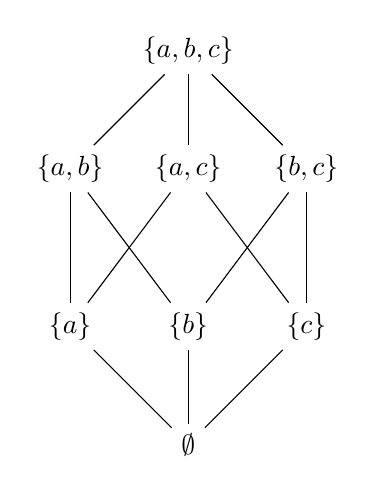
\begin{tikzpicture}
				\node (max) at (0, 5)		{$\{a, b, c\}$};
				\node (d1)   at (-1.5,3.5)	{$\{a, b\}$};
				\node (d2)   at (0,3.5)		 {$\{a, c\}$};
				\node (d3)   at (1.5,3.5)   {$\{b, c\}$};
				\node (a)   at (-1.5,1.5)	  {$\{a\}$};
				\node (b)   at (0,1.5)			{$\{b\}$};
				\node (c)   at (1.5,1.5)        {$\{c\}$};
				\node (min)   at (0, 0)  {$\emptyset$};
				
				\draw (min) -- (a);
				\draw (min) -- (b);
				\draw (min) -- (c);
				\draw (a) -- (d1);
				\draw (a) -- (d2);
				\draw (b) -- (d1);
				\draw (b) -- (d3);
				\draw (c) -- (d2);
				\draw (c) -- (d3);
				\draw (d1) -- (max);
				\draw (d2) -- (max);
				\draw (d3) -- (max);
				%\draw[preaction={draw=white, -,line width=6pt}] (a) -- (e) -- (c);
			\end{tikzpicture}
			\label{fig:DiagramaHasse3-A}
		}\quad\quad\quad %espaco separador
		\subfloat[Representação em forma de quase cubo.]{
			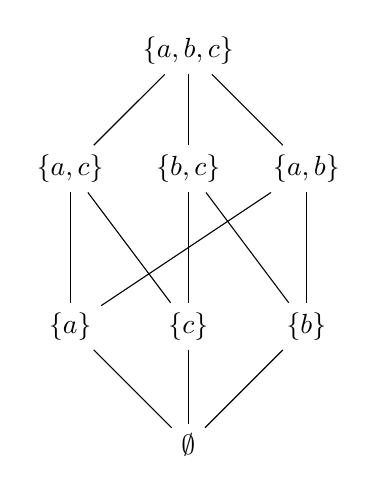
\begin{tikzpicture}
				\node (max) at (0, 5)		{$\{a, b, c\}$};
				\node (d1)   at (-1.5,3.5)	{$\{a, c\}$};
				\node (d2)   at (0,3.5)		 {$\{b, c\}$};
				\node (d3)   at (1.5,3.5)   {$\{a, b\}$};
				\node (a)   at (-1.5,1.5)	  {$\{a\}$};
				\node (b)   at (0,1.5)			{$\{c\}$};
				\node (c)   at (1.5,1.5)        {$\{b\}$};
				\node (min)   at (0, 0)  {$\emptyset$};
				
				\draw (min) -- (a);
				\draw (min) -- (b);
				\draw (min) -- (c);
				\draw (a) -- (d1);
				\draw (a) -- (d3);
				\draw (b) -- (d1);
				\draw (b) -- (d2);
				\draw (c) -- (d2);
				\draw (c) -- (d3);
				\draw (d1) -- (max);
				\draw (d2) -- (max);
				\draw (d3) -- (max);
				%\draw[preaction={draw=white, -,line width=6pt}] (a) -- (e) -- (c);
			\end{tikzpicture}
			\label{fig:DiagramaHasse3-B}
		}
		\caption{Diagramas de Hasse para o \textit{poset} $\langle \wp(\{a, b, c\}), \subseteq \rangle$.}
		\label{fig:DiagramaHasse3}
	\end{figure}
\end{example}

\begin{example}\label{exe:PosetCadeia}
	O \textit{poset} $\langle \{5, 6, 7, 8, 9\}, \leq \rangle$ é representado pelo diagrama a seguir.
	
	\begin{figure}[h]
		\centering
		\begin{tikzpicture}
			\node (min)   at (0, 0)  {$5$};
			\node (1)   at (0, 1.5)  {$6$};
			\node (2)   at (0, 3)  {$7$};
			\node (3)   at (0, 4.5)  {$8$};
			\node (4)   at (0, 6)  {$9$};
			
			\draw (min) -- (1) -- (2) -- (3) -- (4);
		\end{tikzpicture}
		\caption{Diagrama de Hasse do \textit{poset} $\langle \{5, 6, 7, 8, 9\}, \leq \rangle$}
		\label{fig:DiagramaHasse4}
	\end{figure}
\end{example}

\begin{note}
	\textit{Posets} cuja ordem é total também são chamados de cadeias (ver \cite{abe1991-TC, morgado1962poset}) e nesse caso o diagrama será uma linha reta com todos os elementos sobre essa linha, exatamente como no Exemplo \ref{exe:PosetCadeia}. O leitor sem saber já usava esse conceito em seus estudo matemáticos a proferir frases como ``a reta real'' ou ``a reta dos números reais''.
\end{note}

Agora obviamente dado um diagrama de Hasse sempre é possível recuperar a estrutura do \textit{poset} do mesmo, isto é, recuperar o conjunto base e a relação de ordem parcial que define o \textit{poset}, a seguir são apresentados alguns exemplos disto.

\begin{example}
	Dado o diagrama de Hasse da Figura \ref{fig:DiagramaHasse5} a seguir,  dado que $6$ está ligado e abaixo de $3$ e $2$ tem-se que $(6,3), (6, 2) \in R$ onde $R$ é uma relação, o mesmo vale para os pares $(3, 5), (2, 4), (5, 1)$  e $(4, 1)$. Desse modo tal figura representa o \textit{poset} $\langle A, R \rangle$ em que $A = \{1, 2, 3, 4, 5, 6\}$ e $R$ corresponde a relação $\{(6,3), (6, 2), (3, 5), (2, 4), (5, 1), (4, 1), (6, 5), (6, 4), (6, 1), (2, 1), (5, 1)\} \cup Id_A$.
	
		\begin{figure}[h]
		\centering
		\begin{tikzpicture}
			\node (min)   at (0, 0)  {$6$};
			\node (1)   at (2, 2)  {$2$};
			\node (2)   at (-2, 2)  {$3$};
			\node (3)   at (2, 4)  {$4$};
			\node (4)   at (-2, 4)  {$5$};
			\node (max)   at (0, 6)  {$1$};
			
			\draw (min) -- (1) -- (3) -- (max);
			\draw (min) -- (2) -- (4) -- (max);
		\end{tikzpicture}
		\caption{Um diagrama de Hasse.}
		\label{fig:DiagramaHasse5}
	\end{figure}
\end{example}

\begin{example}
	Dado o diagrama de Hasse da Figura \ref{fig:DiagramaHasse6} a seguir representa o \textit{poset} $\langle B, R_B \rangle$ em que $B = \{0, 1, 2, 3, 4, 5, 6\}$ e $R_B = Id_B \cup \{(5, 1), (6, 1), (1, 2), (5, 2), (6, 2), (2, 3), (2, 4), (1, 3), (1, 4)\}$.
	
	\begin{figure}[h]
		\centering
		\begin{tikzpicture}
			\node (min1)   at (2, 0)  {$6$};
			\node (min2)   at (-2, 0)  {$5$};
			\node (1)   at (0, 1)  {$1$};
			\node (2)   at (0, 3)  {$2$};
			\node (max1)   at (2, 4)  {$4$};
			\node (max2)   at (-2, 4)  {$3$};
			\node (min3) at (4, 0) {$0$};
			
			\draw (min1) -- (1) -- (2) -- (max1);
			\draw (min2) -- (1);
			\draw (2) -- (max2);
		\end{tikzpicture}
		\caption{Um diagrama de Hasse.}
		\label{fig:DiagramaHasse6}
	\end{figure}
\end{example}

Como dito em \cite{carmo2013} um \textit{poset} é uma estrutura relacional ordenado, ou ainda, uma álgebra\footnote{O conceito de álgebra será melhor formalizado em capítulos futuros deste manuscrito, por hora o leitor pode pensar em uma álgebra como uma estrutura.} relacional\footnote{Uma álgebra relacional é uma estrutura criada na interseção da lógica de primeira ordem e da álgebra booleana (ou álgebra de conjuntos) finita, tal tipo de álgebra é de suma importância para a área de banco de dados.}, e como uma álgebra pode-se estudar: os elementos destacados, suas sub-álgebras (sub-estruturas) ou ainda os mecanismo de extensão da mesma. Na próxima seção este manuscrito irá realizar um estudo sobre os pontos.

\section{Elementos Notáveis de um \textit{Poset}}\label{sec:ElementosNotaveisPoset}

Como muito bem aprofundado em \cite{carmo2013, morgado1962poset, neggers1998poset}, existem diverso conceitos e aplicações interessantes ligados a ideia de \textit{posets}, assim para ajudar que leitor tenha uma formação sólida na área de teoria dos \textit{posets} é interessante apresentar alguns deste conceitos chaves da teoria, neste seção serão trabalhos os elementos notáveis existes nos \textit{posets} e suas propriedades.

\begin{definition}[Máximo e Mínimo de um subconjunto]\label{def:MaxMinPoset}
	Seja $\langle A, \sqsubseteq \rangle$ um \textit{poset} e $X \subseteq A$ o máximo de $X$, denotado por $max(X)$, é um elemento $x \in X$ tal que para todo $y \in X$ tem-se que $y \sqsubseteq x$. O mínimo de $X$, denotado por $min(X)$,  é um elemento $x \in X$ tal que  para todo $y \in X$ tem-se que $x \sqsubseteq y$.
\end{definition}

\begin{example}
	Considere o \textit{poset} da Figura \ref{fig:DiagramaHasse1} para o conjunto $X = \{1, 2, a\}$ tem-se que $min(X) = 1$ e $max(X) = 2$.
\end{example}

\begin{example}
	Considere o \textit{poset} da Figura \ref{fig:DiagramaHasse2} para o conjunto $X = \{0, 1\}$ tem-se que $min(X) = 0$ e $max(X) = 1$.
\end{example}

\begin{example}
	Considere o \textit{poset} da Figura \ref{fig:DiagramaHasse3-A} para o conjunto $X = \{\{a, b\}, \{a\}, \{b\}, \emptyset\}$ tem-se que $min(X) = \emptyset$ e $max(X) = \{a, b\}$.
\end{example}

Agora é conveniente ressaltar que tanto máximo quando o mínimo podem vir há não existir, isto é, dado um \textit{poset} $\langle A, \sqsubseteq \rangle$ um subconjunto $X$ de $A$ pode-se de tal forma que ele não contenha máximo e(ou) mínimo.

\begin{example}
	Considere o \textit{poset} ilustrado pela Figura \ref{fig:DiagramaHasse5} o subconjunto $\{3, 2, 5, 4\}$ deste \textit{poset} não apresenta máximo e nem mínimo.
\end{example}

\begin{example}
	Considere o \textit{poset} ilustrado pela Figura \ref{fig:DiagramaHasse6} o subconjunto $\{1, 5, 6\}$ deste \textit{poset} possui máximo mas não possui mínimo.
\end{example}

\begin{theorem}[Unicidade do máximo]\label{teo:UnicidadeMaximoPoset}
	Seja $\langle A, \sqsubseteq \rangle$ um \textit{poset} e $X \subseteq A$. Se existe $x \in X$ tal que $max(X) = x$, então $x$ é único.
\end{theorem}

\begin{proof}
	Dado $\langle A, \sqsubseteq \rangle$ um \textit{poset} e $X \subseteq A$. Suponha por absurdo que existem $x, x' \in X$ tal que $max(X) = x$ e $max(X) = x'$ com $x \neq x'$, logo por definição para todo $a \in X$ tem-se que $a \sqsubseteq x$ e $a \sqsubseteq x'$, mas desde que $x, x '\in X$ tem-se que $x \sqsubseteq x'$ e $x' \sqsubseteq x$ e, desde que, $\sqsubseteq$ é antissimétrica tem-se que $x = x'$ o que contradiz a hipótese e, portanto, se existe o máximo de $X$ ele é único.
\end{proof}

\begin{theorem}[Unicidade do mínimo]\label{teo:UnicidadeMinimoPoset}
	Seja $\langle A, \sqsubseteq \rangle$ um \textit{poset} e $X \subseteq A$. Se existe $x \in X$ tal que $min(X) = x$, então $x$ é único.
\end{theorem}

\begin{proof}
	Similar a demonstração do Teorema \ref{teo:UnicidadeMaximoPoset}.
\end{proof}

\begin{theorem}\label{teo:MonotonicidadeInclusaoMaxMin}
	Seja $\langle A, \sqsubseteq \rangle$ um \textit{poset} e $X, Y \subseteq A$ com $X \subseteq Y$ tem-se que:
	\begin{itemize}
		\item[(i)] Se $max(X) = a$ e $max(Y) = b$, então $a \sqsubseteq b$.
		\item[(ii)] Se $min(X) = a$ e $min(Y) = b$, então $b \sqsubseteq a$.
	\end{itemize}
\end{theorem}

\begin{proof}
	A demonstração é simples e fica como exercício ao leitor.
\end{proof}

Além da ideia de máximo e mínimo sobre os \textit{posets} também definido a ideia de maximais e minimais.

\begin{definition}[Elementos maximais]\label{def:MaximaisPoset}
	Seja $\langle A, \sqsubseteq \rangle$ um \textit{poset}  um elemento $x \in A$ é dito ser um maximal se para todo $y \in A$ tem-se que se $x \sqsubseteq y$, então $x = y$.
\end{definition}

\begin{example}
	Considere o \textit{poset} esboçado pela Figura \ref{fig:DiagramaHasse7} a seguir. Para tal \textit{poset} tem-se que o elemento $g$ é um maximal e também é o máximo do conjunto.
	
	\begin{figure}[h]
		\centering
		\begin{tikzpicture}
			\node (a)   at (0, 0)  {$a$};
			\node (b) at (1, 1) {$b$};
			\node (c) at (2, 2) {$c$};
			\node (d) at (-2, 2) {$d$};
			\node (e) at (0, 2) {$e$};
			\node (f) at (1, 3) {$f$};
			\node (g) at (0, 4) {$g$};
			
			\draw (a) -- (b) -- (c);
			\draw (a) -- (d) -- (g);
			\draw (c) -- (f) -- (g);
			\draw (b) -- (e);
			\draw (e) -- (f);
		\end{tikzpicture}
		\caption{Um \textit{poset} representado por um diagrama de Hasse.}
		\label{fig:DiagramaHasse7}
	\end{figure}
\end{example}

\begin{example}
	Considere o \textit{poset} esboçado pela Figura \ref{fig:DiagramaHasse5}. Para tal \textit{poset} tem-se que o elemento $1$ é um maximal e também é o máximo do conjunto.
\end{example}

Em algumas situações elementos maximais coincidem com o máximo, entretanto, como mostrado a seguir ser maximal não é garantia de ser o máximo do conjunto.

\begin{example}
	Considere o \textit{poset} esboçado pela Figura \ref{fig:DiagramaHasse8} a seguir. Para tal \textit{poset} tem-se que os elementos $4$ e $5$ satisfazem a Definição \ref{def:MaximaisPoset} logo ambos são maximais do conjunto, porém, ambos são incomparáveis, portanto, não nenhum é o máximo do conjunto.
	
	\begin{figure}[h]
		\centering
		\begin{tikzpicture}
			\node (1)   at (0, 0)  {$1$};
			\node (2)   at (-1, 1)  {$2$};
			\node (3)   at (1, 1)  {$3$};
			\node (4)   at (0, 2)  {$4$};
			\node (5)   at (2, 2)  {$5$};
			
			\draw (1) -- (2) -- (4);
			\draw (1) -- (3) -- (4);
			\draw (3) -- (5);
		\end{tikzpicture}
		\caption{Um \textit{poset} representado por um diagrama de Hasse.}
		\label{fig:DiagramaHasse8}
	\end{figure}
\end{example} 

De forma dual ao conceito de maximal pode-se definir a ideia de elemento minimal, e isto é feito como se segue.

\begin{definition}[Elementos minimais]\label{def:MinimalPoset}
	Seja $\langle A, \sqsubseteq \rangle$ um \textit{poset}  um elemento $x \in A$ é dito ser um minimal se para todo $y \in A$ tem-se que se $y\sqsubseteq x$, então $x = y$.
\end{definition}

\begin{example}
	Considerando o \textit{poset} da Figura \ref{fig:DiagramaHasse7} tem-se que o elemento $a$ é minimal de tal conjunto e também apresenta a característica de ser o mínimo.
\end{example}

\begin{example}
	Considerando o \textit{poset} da Figura \ref{fig:DiagramaHasse8} tem-se que o elemento $1$ é minimal de tal conjunto e também apresenta a característica de ser o mínimo.
\end{example}

\begin{example}
	Considerando o \textit{poset} da Figura \ref{fig:DiagramaHasse6} tem-se que os elementos $5$ e $6$ são ambos minimais, porém, como são ambos incomparáveis tem-se que nenhum dos dois é o mínimo do conjunto base do \textit{poset}.
\end{example}

\begin{example}
	Considere o \textit{poset} da Figura \ref{fig:DiagramaHasse9} a seguir, tem-se que $g$ e $f$ são elementos maximais e $c, a$ e $b$ são elementos minimais, note que tal \textit{poset} não possui máximo e mínimo.
	
	\begin{figure}[h]
		\centering
		\begin{tikzpicture}
			\node (a)   at (0, 0)  {$a$};
			\node (b)   at (2, 0)  {$b$};
			\node (c)   at (-2, 0)  {$c$};
			\node (d)   at (0, 1)  {$d$};
			\node (e)   at (0, 2)  {$e$};
			\node (f)   at (1, 3)  {$f$};
			\node (g)   at (-1, 3)  {$g$};
			
			\draw (d) -- (c);
			\draw (d) -- (a);
			\draw (d) -- (b);
			\draw (d) -- (e);
			\draw (e) -- (g);
			\draw (e) -- (f);
		\end{tikzpicture}
		\caption{Um \textit{poset} representado por um diagrama de Hasse.}
		\label{fig:DiagramaHasse9}
	\end{figure}
\end{example}

\begin{definition}[Majorante]\label{def:Majorante}
	Seja $\langle A, \sqsubseteq \rangle$ um \textit{poset} e $X \subseteq A$, um elemento $x \in A$ é dito ser um majorante (ou cota superior) de $X$ sempre que para todo $y \in X$ tem-se que $y\sqsubseteq x$.
\end{definition}

\begin{example}
	Considere o \textit{poset} esboçado na Figura \ref{fig:DiagramaHasse9} e o subconjunto $X = \{e, d, c\}$ tem-se que os elementos $e, f$ e $g$ são todos majorantes de $X$. Já os subconjuntos $Y = \{g, f, e\}$ e $Z = \{g, f, a\}$ não possuem majorantes.
\end{example}

\begin{example}
	Considere o \textit{poset} esboçado na Figura \ref{fig:DiagramaHasse8} e o subconjunto $X = \{2, 3, 5\}$  não possui majorantes, já o conjunto $Y = \{1,2, 3, 4\}$ possui o elemento $4$ como majorante.
\end{example}

\begin{example}
	Considere o \textit{poset} esboçado na Figura \ref{fig:DiagramaHasse7} e o subconjunto $X = \{d, e, f\}$ tem-se que o elemento $g$ é o majorante de $X$.
\end{example}

Como mencionado em \cite{abe1991-TC} se $x$ é um majorante (ou cota superior) de um conjunto $X$, é dito que $X$ é um conjunto majorado pelo elemento $x$ ou que o conjunto $X$ possui uma cota superior $x$.

\begin{definition}[Conjunto dos majorantes]\label{def:ConjuntoDosMajorantes}
	Seja $\langle A, \sqsubseteq \rangle$ um \textit{poset} e $X \subseteq A$, o conjunto de todos os majorantes de $X$ é denotado por $X_\curlywedge$.
\end{definition}

Como dito em \cite{abe1991-TC, carmo2013, morgado1962poset} a maior parte dos conceito na teoria dos \textit{posets} tem natureza dual, assim é natural que seja imediatamente apresentadas as definições de minorantes e conjunto dos minorantes.

\begin{definition}[Minorante]\label{def:Mjnorante}
	Seja $\langle A, \sqsubseteq \rangle$ um \textit{poset} e $X \subseteq A$, um elemento $x \in A$ é dito ser um minorante (ou cota inferior) de $X$ sempre que para todo $y \in X$ tem-se que $x\sqsubseteq y$.
\end{definition}

\begin{example}
	Considere o \textit{poset} esboçado na Figura \ref{fig:DiagramaHasse9} e o subconjunto $X = \{e, d, c\}$ tem-se que o elemento $c$ é o minorante de $X$. Já os subconjuntos $Y = \{g, f, e\}$ tem como minorantes os elementos $e, d, c, a$e $b$, por fim, para o conjunto $Z = \{g, f, a\}$ o único minorantes é o elemento $a$.
\end{example}

\begin{example}
	Considere o \textit{poset} esboçado na Figura \ref{fig:DiagramaHasse8} e o subconjunto $X = \{2, 3, 5\}$  tem como minorante o elemento $1$, já o conjunto $Y = \{3, 4, 5\}$ possui como minorantes os elementos $1$ e $3$.
\end{example}

\begin{example}
	Considere o \textit{poset} esboçado na Figura \ref{fig:DiagramaHasse7} e o subconjunto $X = \{d, e, f\}$ tem-se que o elemento $a$ é o único minorante deste conjunto, já para o conjunto $Y = \{g, f\}$ tem-se os elementos $f, e, c, b$ e $a$ como minorantes de $Y$.
\end{example}

\begin{definition}[Conjunto dos minorantes]\label{def:ConjuntoDosMjnorantes}
	Seja $\langle A, \sqsubseteq \rangle$ um \textit{poset} e $X \subseteq A$, o conjunto de todos os minorantes de $X$ é denotado por $X_\curlyvee$.
\end{definition}

\begin{theorem}
	Seja $\langle A, \sqsubseteq \rangle$ um \textit{poset} e $X \subset A$. Se $a \in A$ é um majorante (minorante) de $X$ e $a \in X$, então $a = max(X)$ $(a = min(X))$.
\end{theorem}

\begin{proof}
	Trivial.
\end{proof}

O próximo resultado estabelece que o conjunto de majorantes e minorantes respeita a monotonicidade da relação inclusão.

\begin{theorem}\label{teo:MonotonicidadeMajoranteMinorante}
	Seja $\langle A, \sqsubseteq \rangle$ um \textit{poset} e $X, Y \subseteq A$. Se $X \subseteq Y$, então: 
	\begin{itemize}
		\item[(i)] $Y_\curlywedge \subseteq X_\curlywedge$.
		\item[(ii)] $Y_\curlyvee \subseteq X_\curlyvee$.
	\end{itemize}
\end{theorem}

\begin{proof}
	A demonstração é simples e ficará como exercício ao leitor. 
\end{proof}

\begin{definition}[Conjunto limitado]\label{def:ConjuntoLimitadoPoset}
	Seja $\langle A, \sqsubseteq \rangle$ um \textit{poset} e $X \subseteq A$, o conjunto $X$ é dito ser limitado em $A$ sempre que $X$ possui majorantes e minorantes.
\end{definition}

\begin{example}
	Considere o \textit{poset} $\langle \mathbb{N}, \leq \rangle$ o conjunto $X_{k_1, k_2} = \{x \in \mathbb{N} \mid k_1 < x < k_2\}$ é um conjunto que sempre possuirá majorantes e minorantes (a saber $k_1$ e $k_2$) logo ele é um conjunto limitado em $\langle \mathbb{N}, \leq \rangle$.
\end{example}

\begin{example}
	Considere o \textit{poset} $\langle \wp(A), \subseteq \rangle$ onde $A$ é um conjunto qualquer, um conjunto $X \in \wp(A)$ sempre irá possuir minorante e majorante, que como dito em \cite{abe1991-TC} são gerados pela interseção e união respectivamente. Assim qualquer $X \in \wp(A)$ sempre será um conjunto limitado em $\langle \wp(A), \subseteq \rangle$.
\end{example}

\begin{example}
	Considere o \textit{poset} esboçado na Figura \ref{fig:DiagramaHasse9} e o subconjunto $X = \{e, d, c, a , b\}$ tem-se que tal conjunto possui os majorantes $e, g$ e $f$, mas não possui minorantes, assim $X$ não é limitado.
\end{example}

\begin{theorem}\label{teo:MinoranteMajoranteInclusao}
	Seja $\langle A, \sqsubseteq \rangle$ um \textit{poset} e $X \subseteq A$. Se $X \neq \emptyset$, então $X \subseteq (X_\curlyvee)_\curlywedge$.
\end{theorem}

\begin{proof}
	Dado $\langle A, \sqsubseteq \rangle$ um \textit{poset} e $X \subseteq A$, suponha que $X \neq \emptyset$, assim para todo $x \in X$ e cada $y \in X_\curlyvee$ tem-se que $y \sqsubseteq x$, logo $x \in (X_\curlyvee)_\curlywedge$, portanto, $X \subseteq (X_\curlyvee)_\curlywedge$.
\end{proof}

\begin{theorem}\label{teo:MajoranteMinoranteInclusao}
	Seja $\langle A, \sqsubseteq \rangle$ um \textit{poset} e $X \subseteq A$. Se $X \neq \emptyset$, então $X \subseteq (X_\curlywedge)_\curlyvee$.
\end{theorem}

\begin{proof}
	Similar a prova do Teorema \ref{teo:MinoranteMajoranteInclusao}.
\end{proof}

\begin{theorem}\label{teo:IdadeMajoranteMinorante}
	Seja $\langle A, \sqsubseteq \rangle$ um \textit{poset} e $X \subseteq A$. Se $X \neq \emptyset$, então:
	\begin{itemize}
		\item[(i)]  $X_\curlywedge = ((X_\curlywedge)_\curlyvee)_\curlywedge$.
		\item[(ii)] $X\curlyvee = ((X_\curlyvee)_\curlywedge)_\curlyvee$.
	\end{itemize}
\end{theorem}

\begin{proof}
	Dado $\langle A, \sqsubseteq \rangle$ um \textit{poset} e $X \subseteq A$. Suponha que $X \neq \emptyset$, assim tem-se que:
	\begin{itemize}
		\item[(i)] Pelo Teorema \ref{teo:MajoranteMinoranteInclusao} segue que $X_\curlywedge \subseteq ((X_\curlyvee)_\curlywedge)_\curlyvee$, por outro lado, pelo Teorema \ref{teo:MinoranteMajoranteInclusao} pode-se concluir que $((X_\curlywedge)_\curlyvee)_\curlywedge \subseteq X_\curlywedge$, portanto, pela Definição \ref{def:IgualdadeConjuntos} tem-se que  $X_\curlywedge = ((X_\curlywedge)_\curlyvee)_\curlywedge$.
		\item[(ii)] Similar ao item anterior.
	\end{itemize}
	Completando assim a prova.
\end{proof}

\begin{theorem}\label{teo:RotacaoMajoranteMinorante}
	Seja $\langle A, \sqsubseteq \rangle$ um \textit{poset} e $X, Y \subseteq A$. Se $X, Y \neq \emptyset$, então:
	\begin{itemize}
		\item[(i)]  $(X \cup Y)_\curlyvee = X_\curlyvee \cap Y_\curlyvee$.
		\item[(ii)] $(X \cup Y)_\curlywedge = X_\curlywedge \cap Y_\curlywedge$.
	\end{itemize}
\end{theorem}

\begin{proof}
	Dado $\langle A, \sqsubseteq \rangle$ um \textit{poset} e $X \subseteq A$. Suponha que $X \neq \emptyset$, assim tem-se que:
	\begin{itemize}
		\item[(i)] Desde que $X \subseteq X \cup Y$ e  $Y \subseteq X \cup Y$ tem-se pelo Teorema \ref{teo:MonotonicidadeMajoranteMinorante} que $(X \cup Y)_\curlyvee \subseteq X_\curlyvee$ e  $(X \cup Y)_\curlyvee \subseteq Y_\curlyvee $, consequentemente, $(X \cup Y)_\curlyvee \subseteq X_\curlyvee \cap Y_\curlyvee$. Por outro lado, para todo $x \in X_\curlyvee \cap Y_\curlyvee$ tem-se para todo $y \in X$ que $x \leq y$ e para todo $z \in Y$ que $x \leq z$, assim $x \in (X \cup Y)_\curlyvee$ e assim $(X \cup Y)_\curlyvee \subseteq X_\curlyvee \cap Y_\curlyvee$ e, portanto, pela Definição \ref{def:IgualdadeConjuntos}  tem-se que $(X \cup Y)_\curlyvee = X_\curlyvee \cap Y_\curlyvee$.
		\item[(ii)] Similar ao item anterior.
	\end{itemize}
	O que termina a prova.
\end{proof}

\begin{definition}[Supremo]\label{def:Supermo}
	Seja $\langle A, \sqsubseteq \rangle$ um \textit{poset} e $X \subseteq A$ o supremo de $X$ (caso exista), denotado por $sup(X)$, é o menor dos majorantes, em notação formal tem-se que $sup(X) = min(X_\curlywedge)$.
\end{definition}

Como dito em \cite{abe1991-TC, carmo2013}, uma forma de caracterização do supremo é através de suas propriedades inerentes, e isto é feito da seguinte forma, dado um \textit{poset} $\langle A, \sqsubseteq \rangle$ tem-se que $sup(X) = a $ se, e somente se:

\begin{itemize}
	\item[1.] $a \in A$.
	\item[2.] Para todo $x \in X$ tem-se que $x \sqsubseteq a$.
	\item[3.] Se $a' \in A$ e para todo $x \in X$ tem-se que  $x \sqsubseteq a'$, então $a \sqsubseteq a'$.
\end{itemize}

Note que a propriedade (1) diz que o supremo (caso exista) é sempre um elemento do poset, já a propriedade (2) estabelece que o supremo deve ser um majorante e a propriedade (3) estabelece que o supremo deve ser a menor cota superior, isto é, o mínimo do conjunto dos majorantes.

\begin{definition}[Ínfimo]\label{def:Infimo}
	Seja $\langle A, \sqsubseteq \rangle$ um \textit{poset} e $X \subseteq A$ o ínfimo de $X$ (caso exista), denotado por $inf(X)$, é o maior dos minorantes, em notação formal tem-se que $sup(X) = max(X_\curlyvee)$.
\end{definition}

Dualmente ao supremo como dito em \cite{abe1991-TC, carmo2013}, uma forma de caracterização do ínfimo é através de suas propriedades inerentes, e isto é feito da seguinte forma, dado um \textit{poset} $\langle A, \sqsubseteq \rangle$ tem-se que $inf(X) = a $ se, e somente se:

\begin{itemize}
	\item[1.] $a \in A$.
	\item[2.] Para todo $x \in X$ tem-se que $a \sqsubseteq x$.
	\item[3.] Se $a' \in A$ e para todo $x \in X$ tem-se que  $a' \sqsubseteq x$, então $a' \sqsubseteq a$.
\end{itemize}

Ou seja, a propriedade (1) diz que o ínfimo (caso exista) é sempre um elemento do poset, já a propriedade (2) estabelece que o  ínfimo deve ser um minorante e a propriedade (3) estabelece que o  ínfimo deve ser a maior cota inferior, isto é, o máximo do conjunto dos minorantes.

\begin{remark}
	Como destacado em \cite{fmcbook}, os termos \textit{least upper bound} (menor cota superior) e \textit{join} são sinônimos de supremo, enquanto, que \textit{greatest lower bound} (maior cota inferior) e \textit{meet} são sinônimos de ínfimo.
\end{remark}

\begin{example}\label{exe:SupremoInfimoPoset}
	Considere o \textit{poset} representado pela Figura \ref{fig:DiagramaHasse10} a seguir, o subconjunto $X = \{2, 3, 4, 5\}$ é tal que $sup(X) = 7$ e $inf(X) = 2$, por lado, para o subconjunto $Y = \{1, 0, 2, 4\}$ tem-se que $sup(Y) = 3$ mas não existe um ínfimo de tal conjunto. Além disso, pegando o conjunto inteiro do \textit{poset} tem-se que o conjunto possui supremo, a saber $7$ mas não possui ínfimo. 
	
	\begin{figure}[h]
		\centering
		\begin{tikzpicture}
			\node (min1)   at (0, 0)  {$1$};
			\node (min2)   at (2, 0)  {$0$};
			\node (a) at (1, 1)  {$2$};
			\node (b)   at (0, 2)  {$4$};
			\node (c)   at (2, 2)  {$5$};
			\node (e) at (1, 3)  {$3$};
			\node (f) at (3, 3)  {$6$};
			\node (g) at (2, 4)  {$7$};
			
			\draw (min1) -- (a) -- (b) -- (e) -- (g);
			\draw (min2) -- (a) -- (c) -- (f) -- (g);
			\draw (c) -- (e);
		\end{tikzpicture}
		\caption{Diagrama de Hasse do \textit{poset} do Exemplo \ref{exe:SupremoInfimoPoset}.}
		\label{fig:DiagramaHasse10}
	\end{figure}
\end{example}

\begin{example}
	Considerando o \textit{poset} $\langle \mathbb{Q}, \leq \rangle$ tem-se que o subconjunto $\{x \in Q \mid x^2 \leq 2\}$ não possui supremo pois $\sqrt{2} \notin \mathbb{Q}$.
\end{example}

\begin{theorem}
	Seja $\langle A, \sqsubseteq \rangle$ um \textit{poset} e $X, Y \subseteq A$. Se $X \subseteq Y$ e além disso $X$ e $Y$ possuem supremo, então $sup(X) \sqsubseteq sup(Y)$.
\end{theorem}

\begin{proof}
	Dado $\langle A, \sqsubseteq \rangle$ um \textit{poset} e $X, Y \subseteq A$, assuma $X \subseteq Y$ e que que $X$ e $Y$ possuem supremo, assim pelo Teorema \ref{teo:MonotonicidadeMajoranteMinorante}(i) tem-se que $Y_\curlywedge \subseteq X_\curlywedge$.  Mas pelo Teorema \ref{teo:MonotonicidadeInclusaoMaxMin}(ii) tem-se que $min(Y_\curlywedge) \sqsubseteq min(X_\curlywedge)$, logo $sup(X) \sqsubseteq sup(Y)$.
\end{proof}

\begin{theorem}
	Seja $\langle A, \sqsubseteq \rangle$ um \textit{poset} e $X, Y \subseteq A$. Se $X \subseteq Y$ e além disso $X$ e $Y$ possuem ínfimo, então $inf(Y) \sqsubseteq inf(X)$.
\end{theorem}

\begin{proof}
	Dado $\langle A, \sqsubseteq \rangle$ um \textit{poset} e $X, Y \subseteq A$, assuma $X \subseteq Y$ e que que $X$ e $Y$ possuem supremo, assim pelo Teorema \ref{teo:MonotonicidadeMajoranteMinorante}(ii) tem-se que $Y_\curlywedge \subseteq X_\curlywedge$.  Mas pelo Teorema \ref{teo:MonotonicidadeInclusaoMaxMin}(i) tem-se que $max(Y_\curlyvee) \sqsubseteq max(X_\curlyvee)$, logo $inf(Y) \sqsubseteq inf(X)$.
\end{proof}

\begin{theorem}\label{teo:InfimoApartirSupremo}
	Se $\langle A, \sqsubseteq \rangle$ é um \textit{poset}, $X \subseteq A$ com $sup(X_\curlyvee) = a$ e $a \in A$, então $inf(X) = sup(X_\curlyvee) $.
\end{theorem}

\begin{proof}
	$\langle A, \sqsubseteq \rangle$ é um \textit{poset}, $X \subseteq A$ com $sup(X_\curlyvee) = a$ e $a \in A$, agora note que para qualquer que seja $x \in X$ e $y \in X_\curlyvee$ tem-se que $y \sqsubseteq x$, e assim $x$ é claramente um majorante de $X_\curlyvee$, ou seja, $x \in (X_\curlyvee)_\curlywedge$,  consequentemente, $a \sqsubseteq y$, uma vez que, $sup(X_\curlyvee) = a$, assim $a$ é um minorante de $X$, ou seja, $a \in X_\curlyvee$. Por outro lado, para qualquer $z \in X_\curlyvee$ tem-se que $z \sqsubseteq a$ e, portanto, $a = inf(X)$.
\end{proof}

\begin{theorem}\label{teo:SupremoApartirInfimo}
	Se $\langle A, \sqsubseteq \rangle$ é um \textit{poset}, $X \subseteq A$ com $inf(X_\curlyvee) = a$ e $a \in A$, então $sup(X) = inf(X_\curlywedge) $.
\end{theorem}

\begin{proof}
	Similar a demonstração do Teorema \ref{teo:InfimoApartirSupremo}.
\end{proof}

\begin{remark}
	Quando um conjunto $X$ satisfaz o Teorema  \ref{teo:InfimoApartirSupremo} é dito que ele é inferiormente limitado, e quando ele satisfaz o Teorema \ref{teo:SupremoApartirInfimo} é dito que ele é superiormente limitado. Quando ele satisfaz os dois então ele satisfaz a Definição \ref{def:ConjuntoLimitadoPoset}.
\end{remark}

\begin{theorem}
	Se $\langle A, \sqsubseteq \rangle$ é um \textit{poset}, então as seguintes asserções são equivalentes:
	\begin{itemize}
		\item[(1)] Todo subconjunto não vazio superiormente limitado de $A$ possui supremo.
		\item[(2)] Todo subconjunto não vazio inferiormente limitado de $A$ possui ínfimo.
	\end{itemize}
\end{theorem}
	
\begin{proof}
	Dado $\langle A, \sqsubseteq \rangle$ um \textit{poset}, tem-se que:
	
	$(1) \Rightarrow (2)$ Assuma que todo subconjunto não vazio superiormente limitado de $A$ possui supremo, agora seja $X \subseteq A$ limitado inferiormente, ou seja, $X_\curlyvee \neq \emptyset$, agora obviamente cada $x \in X$ é tal que $x$ é um majorante de $X_\curlyvee$, ou seja, $x \in (X_\curlyvee)_\curlywedge$ e, portanto, $X_\curlyvee$ é superiormente limitado, logo pelo Teorema \ref{teo:SupremoApartirInfimo} existe o supremo do conjunto $X_\curlyvee$, consequentemente pelo Teorema \ref{teo:InfimoApartirSupremo} existe o ínfimo de $X_\curlyvee$.
	
	$(2) \Rightarrow (1)$ Similar ao item anterior.
\end{proof}

\section{Princípio da Boa Ordenação}

Escrever depois...

\section{Somas Ordinais, Ordem Produto e Ordem Lexicográfica}\label{sec:OperacoesPoset}

Escrever depois...

\section{Questionário}\label{sec:Questionario4part1}

\begin{problem}\label{prob:EquivalenciaOrdem1}
	Seja $B$ o conjunto de todos os brasileiros e $R$ uma relação definida sobre $B$ como $x \mathrel{R}$ se, e somente se, $x$ e $y$ são nascidos no mesmo estado ou território do Brasil. Responda as questões a seguir.
\end{problem}

\begin{exerList}
	\item Quantas classes de equivalência diferentes são determinadas por $R$?
	\item Escreva em notação compacta a classe de equivalência definida por Heitor Villa-Lobos.
	\item Responda se Getúlio Vargas $\in$ [Heitor Villa-Lobos].
	\item Escreva em notação compacta a classe de equivalência definida por Leopoldo Nachbin.
\end{exerList}

\begin{problem}\label{prob:EquivalenciaOrdem2}
	Considerando o conjunto $A = \mathbb{N}^2$ demonstre que a relação $R = \{((a, b), (c, d)) \mid a+b = c+d\}$ é uma relação de equivalência sobre $A^2$.
\end{problem}

\begin{problem}\label{prob:EquivalenciaOrdem3}
	Considerando os conjuntos e as relações de equivalência a seguir sobre tais conjuntos, esboce os conjuntos quociente formado por cada relação.
\end{problem}

\begin{exerList}
	\item $A = \{a,b,c,d,e \}$ e $R =\{(a,a),(a,e),(b,b),(b,d),(c,c),(d,b),(d,d), (e, a), (e, e)\}$.
	\item $C = \{1, 2, 3, 4\}$ e $S = \{(1, 1), (2, 2), (3, 3), (4, 4), (2, 4), (4, 2)\}$.
	\item $A = \{x \in \mathbb{N} \mid x \leq 20\}$ e $K = \{(x, y) \in A^2 \mid (\exists k \in \mathbb{N})[[\displaystyle\frac{(x - y)}{4} = k]\}$.
	\item $D = \{x \in \mathbb{Z} \mid -4 \leq x \leq 5\}$ e $T = \{(x, y) \in D^2 \mid (\exists k \in \mathbb{Z})[\displaystyle\frac{(x - y)}{3} = k]\}$.
	\item $E = \{(1, 3), (2,4), (0, 3), (-4, -8), (3, 9), (-1, 5), (2, -4), (1, 5), (3, 6)\}$ e $L$ é a relação definida sobre $E$ da seguinte forma $(x_1, y_1) \mathrel{L} (x_2, y_2)$ se, e somente se, $x_0y_1 = x_1y_0$.
	\item $A = \{-1, 0, 1\}$ e $M = \{(X, Y) \in \wp(A) \mid num(X) = num(Y)\}$ em que $num(D)$ é o número de elementos em $D$ para qualquer $D \in \wp(A)$.
	\item $N = \{1, -2, 3\}$ e $M = \Big\{(X, Y) \in \wp(N) \mid \displaystyle\sum_{x \in X} x = \displaystyle\sum_{y \in Y} y\Big\}$ em que $\displaystyle\sum_{a \in D} a$  representa a soma de todo os elementos $a$ pertencentes ao conjunto $D$ para qualquer que seja o $D \in \wp(N)$.
	\item $D = \{x \in \mathbb{Z} \mid -5 \leq x \leq 5\}$ e $T = \{(x, y) \in D^2 \mid (\exists k \in \mathbb{Z})[\displaystyle\frac{(x^2 - y^2)}{3} = k]\}$.
	\item $F = \{x \in \mathbb{Z} \mid -4 \leq x \leq 5\}$ e $T = \{(x, y) \in F^2 \mid (\exists k \in \mathbb{Z})[\displaystyle\frac{(x^2 - y^2)}{3} = k]\}$.
	\item $B = \{00, 01, 02, 10, 11, 12, 20, 21, 22\}$ $R = \{(x, y) \in B^2 \mid  sC(x) = sC(y)\}$ onde $sC(x)$ denotada a soma dos caracteres para qualquer $x \in B$.
\end{exerList}

\begin{problem}\label{prob:EquivalenciaOrdem4}
	Seja $A$ o conjunto de todos os estudantes do seu campus demonstre que a relação $T$ definida sobre $A$ como ``$x \mathrel{T} y$ se, e somente se, $x$ é do mesmo curso que $y$'' é uma relação de equivalência.
\end{problem}

\begin{problem}\label{prob:EquivalenciaOrdem5}
	Seja $A = \{a, b, c, d\}$ e $R = \{(a, a), (a, b), (b, a), (b, b), (c, d), (d, c), (d,d), (c, c)\}$. Prove que $R$ é uma relação de equivalência sobre $A$ e esboce também o espaço quociente $A_{/_R}$.
\end{problem}

\begin{problem}\label{prob:EquivalenciaOrdem6}
	Sendo $R$ uma relação de equivalência sobre $X$ é correto afirma que $dom(R) = X$?
\end{problem}

\begin{problem}\label{prob:EquivalenciaOrdem7}
	Suponha que  $R$ e $S$ são duas relações de equivalência sobre um conjunto $A$. Prove que $R \cap S$ é também uma relação de equivalência sobre $A$.
\end{problem}

\begin{problem}\label{prob:EquivalenciaOrdem8}
	Demonstre que a relação $R = \{(x, y) \in \mathbb{Z}^2 \mid x - y \in \mathbb{Z} \}$ é uma relação de equivalência sobre o conjunto $\mathbb{Z}$.
\end{problem}

\begin{problem}\label{prob:EquivalenciaOrdem9}
	Considerando para todo $n \in \mathbb{Z}$ realize o que é solicitado a seguir.
\end{problem}

\begin{exerList}
	\item Demonstre que $R_n = \{(x, y) \in \mathbb{Z}^2 \mid \displaystyle\frac{x - y}{n} = k\}$ é uma relação de equivalência.
	\item Para o caso particular de $n = 2$ esboce usando notação compacta a classe $[1]$ com respeito a relação $R_n$.
	\item Para o caso particular de $n = 5$ esboce usando notação compacta a classe $[-4]$ com respeito a relação $R_n$.
\end{exerList}

\begin{problem}\label{prob:EquivalenciaOrdem10}
	Sejam $A = \{1, 2\}$ e $B = \{3, 4\}$ dois elementos de uma partição de $\{1, 2, 3, 4\}$ liste os pares ordenados que compõem a relação de equivalência que definiu a partição que contém $A$ e $B$.
\end{problem}

\begin{problem}\label{prob:EquivalenciaOrdem11}
	Demonstre que a relação $P = \{(x, y) \in \mathbb{Z}^2 \mid (\exists k \in \mathbb{Z})[x^2 - y^2 = 2k]\}$ é uma relação de equivalência sobre o conjunto $\mathbb{Z}$ e usando notação compacta a classe escreve o espaço quociente gerado por tal relação.
\end{problem}

\begin{problem}\label{prob:EquivalenciaOrdem12}
	Seja $S = \mathbb{N}^2$. Demonstre que a relação $P = \{((x, y), (w, z)) \in S^2 \mid x = z \}$ é uma relação de equivalência sobre o conjunto $S$ e usando notação compacta a classe escreve o espaço quociente gerado por tal relação.
\end{problem}

\begin{problem}\label{prob:EquivalenciaOrdem13}
	Seja $S = \mathbb{Z}^2$. Verifique se a relação $T = \{((x, y), (w, z)) \in S^2 \mid x - y = w - z \}$ é uma relação de equivalência sobre o conjunto $S$, se for então usando notação compacta a classe escreve o espaço quociente gerado por tal relação.
\end{problem}

\begin{problem}\label{prob:EquivalenciaOrdem14}
	Verifique se as seguintes estruturas são \textit{posets}.
\end{problem}

\begin{exerList}
	\item $\langle \mathbb{N}, \alpha \rangle$ onde $\alpha = \{(x, y) \in \mathbb{N}^2 \mid \text{ o resto da divisão de $y$ por $x$ é igual a } 1\}$.
	\item $\langle \mathbb{Z}, \alpha \rangle$ onde $\alpha = \{(x, y) \in \mathbb{Z}^2  \mid y = x + 3\}$.
	\item $\langle \mathbb{N}, \alpha \rangle$ onde $\alpha = \{(x, y) \in \mathbb{N}^2  \mid y - x \in \mathbb{N}\}$.
	\item $\langle \mathbb{Z}, \alpha \rangle$ onde $\alpha = \{(x, y) \in \mathbb{Z}^2  \mid 2y - x \in \mathbb{N}\}$.
\end{exerList}

\begin{problem}\label{prob:EquivalenciaOrdem15}
	Para cada \textit{poset} a seguir desenhe o diagrama um Hasse para o mesmo.
\end{problem}

\begin{exerList}
	\item $\langle \{1, 2, 3, 4, 5, 6, 10, 15, 20, 60\}, M \rangle$ onde $x \mathrel{M} y$ se, e somente se, $\displaystyle\frac{60}{x} = y$.
	\item $\langle \{1, 2, 3, 4, 5, 6, 7, 8, 9, 10\}, D\rangle$ onde $x \mathrel{D} y$ se, e somente se, $\displaystyle\frac{y}{x} = k$ tal que $k \in \{1, 2, 3, 4, 5, 6, 7, 8, 9, 10\}$.
	\item $\langle \{1, 2, 3\}, \{(1, 1), (1, 2), (2, 2), (3, 3), (1, 3), (2, 3)\} \rangle$.
	\item $\langle \{a, b, c, d\}, \{(d, d), (b, b), (a, a), (c, c), (d, c), (d, a), (a, c)\} \rangle$.
\end{exerList}

\begin{problem}\label{prob:EquivalenciaOrdem16}
	Para cada um dos diagrama na Figura \ref{fig:DiagramaExercicioPoset1},   construa sua estrutura de \textit{poset}.
\end{problem}

\begin{figure}[h]
	\centering
	\subfloat[]{
		\begin{tikzpicture}
			\node (max1)  at  (0, 4){$1$};
			\node (max2)  at  (2, 4){$2$};
			\node (max3)  at  (4, 4){$3$};
			
			\node (mid1)  at  (0, 2){$7$};
			\node (mid2)  at  (2, 2){$8$};
			\node (mid3)  at  (4, 2){$9$};
			
			\node (min1)  at  (0, 0){$4$};
			\node (min2)  at  (2, 0){$5$};
			\node (min3)  at  (4, 0){$6$};
			
			\draw (min1) -- (mid1) -- (max1);
			\draw (min2) -- (mid2) -- (max2);
			\draw (min3) -- (mid3) -- (max3);
			%\draw[preaction={draw=white, -,line width=6pt}] (a) -- (e) -- (c);
		\end{tikzpicture}
		\label{fig:DiagramaHasseExe-A}
	}\quad\quad\quad %espaco separador
	\subfloat[]{
		\begin{tikzpicture}
			\node (max) at (0, 5)		{$101$};
			
			\node (mid1)  at  (-2, 2)   {$011$};
			\node (mid2)  at  (2, 1)   {$110$};
			\node (mid3)  at  (0, 3)   {$001$};
			
			\node (min) at (0,0)       {$111$};
			
			\draw (min) -- (mid1) -- (max);
			\draw (min) -- (mid2) -- (mid3) -- (max);
			%\draw[preaction={draw=white, -,line width=6pt}] (a) -- (e) -- (c);
		\end{tikzpicture}
		\label{fig:DiagramaHasseExe-B}
	}
	\caption{Diagramas de Hasse para a questão \ref{prob:EquivalenciaOrdem15}.}
	\label{fig:DiagramaExercicioPoset1}
\end{figure}


\begin{problem}\label{prob:EquivalenciaOrdem17}
	Considere o conjunto $X = \{a, b, c, d, e, f, g, h, i\}$ e $R$ a relação de ordem parcial representada pela Figura \ref{fig:ExercicioDePoset17}, calcule o máximo, mínimo, elementos maximais, elementos minimais, conjuntos dos majorantes, conjuntos dos minorantes, supremo e ínfimo dos seguintes subconjuntos  de $X$:
\end{problem}

\begin{figure}[h]
	\centering
	\begin{tikzpicture}
		\node (a) at (0, 0)		{$a$};
		\node (b) at (1, 1)		{$b$};
		\node (c) at (-1, 1)		{$c$};
		\node (f) at (2, 2)		{$f$};
		\node (e) at (0, 2)		{$e$};
		\node (d) at (-2, 2)		 {$d$};
		\node (h) at (1, 3)		{$h$};
		\node (g) at (-1, 3)		{$g$};
		\node (i) at (0, 4)		 {$i$};
		
		\draw (a) -- (b) -- (f) -- (h) -- (i);
		\draw (a) -- (c) -- (d) -- (g) -- (i);
		\draw (c) -- (e) -- (h);
		\draw (b) -- (e) -- (g);
		%\draw[preaction={draw=white, -,line width=6pt}] (a) -- (e) -- (c);
	\end{tikzpicture}
	\caption{Legenda}
	\label{fig:ExercicioDePoset17}
\end{figure}

\begin{exerList}
	\item $A_1 = \{d, e, b\}$.
	\item $A_2= \{a, c, e, b\}$.
	\item $A_3 = \{g, e, h\}$.
	\item $A_4 = \{d, e, f\}$.
	\item $A_5 = \{a, c, f\}$.
	\item $A_6 = \{a, e\}$.
	\item $A_7 = \{i\}$.
	\item $A_8 = \{d, f, a, i\}$.
	\item $A_9 = \{g, c, b, h\}$.
	\item $A_{10} = \{a, c, f, e\}$.
\end{exerList}

\begin{problem}\label{prob:EquivalenciaOrdem18}
	Considere o conjunto $X = \{0, 1, 2, 3, 4, 5, 6, 7, 8, 9, 10\}$ e $R$ a relação de ordem parcial representada pela Figura \ref{fig:ExercicioDePoset18}, calcule o máximo, mínimo, elementos maximais, elementos minimais, conjuntos dos majorantes, conjuntos dos minorantes, supremo e ínfimo dos seguintes subconjuntos  de $X$:
\end{problem}

\begin{figure}[h]
	\centering
	\begin{tikzpicture}
		\node (a) at (0, 0)		{$1$};
		\node (b) at (1, 1)		{$2$};
		\node (c) at (-1, 1)		{$3$};
		\node (f) at (2, 2)		{$4$};
		\node (e) at (0, 2)		{$5$};
		\node (d) at (-2, 2)		 {$10$};
		\node (d1) at (-3, 1)		 {$6$};
		\node (h) at (1, 3)		{$9$};
		\node (h1) at (2, 4)		{$0$};
		\node (g) at (-1, 3)		{$8$};
		\node (i) at (0, 4)		 {$7$};
		
		\draw (a) -- (b) -- (f) -- (h) -- (i);
		\draw (a) -- (c) -- (d) -- (g) -- (i);
		\draw (c) -- (e) -- (h);
		\draw (b) -- (e) -- (g);
		\draw (d1) -- (d);
		\draw (h) -- (h1);
		%\draw[preaction={draw=white, -,line width=6pt}] (a) -- (e) -- (c);
	\end{tikzpicture}
	\caption{Legenda}
	\label{fig:ExercicioDePoset18}
\end{figure}

\begin{exerList}
	\item $A_1 = \{10, 2, 9\}$.
	\item $A_2= \{0, 6, 4\}$.
	\item $A_3 = \{10, 3, 6, 7\}$.
	\item $A_4 = \{6, 7, 0, 1\}$.
	\item $A_5 = \{9, 8, 3, 2\}$.
	\item $A_6 = \{5, 8, 2\}$.
	\item $A_7 = \{3, 9, 5, 2\}$.
	\item $A_8 = \{10, 1, 4, 7\}$.
	\item $A_9 = \{0,  9, 4, 8\}$.
	\item $A_{10} = \{6, 10, 9, 3, 0, 7\}$.
\end{exerList}

\begin{problem}\label{prob:EquivalenciaOrdem19}
	Considere um conjunto $A$ qualquer e uma relação binária $R$ sobre $A$ demonstre que $R$ será uma relação de ordem parcial e de equivalência simultaneamente se, e somente se, $R$ for a relação de identidade em $A$.
\end{problem}

\begin{problem}\label{prob:EquivalenciaOrdemXX}
	Dê exemplo de:
\end{problem}

\begin{exerList}
	\item Duas relação de ordem parcial sobre um conjunto $A$, tal que a união das duas não seja uma ordem parcial sobre $A$.
	\item Duas relação de ordem parcial sobre um conjunto $A$, tal que a composição das duas não seja uma ordem parcial sobre $A$.
\end{exerList}
